\begin{figure}
    \centering
    \begin{subfigure}{0.4\linewidth}
        
\includegraphics[width=\linewidth]{images/pruning/per_method/WeaknessIntoStrength_pruning_per_method_maximal_pr_rate.eps}
        \caption{WeaknessIntoStrength}
        \label{fig:pruning-max-pr-rate-weakness}
    \end{subfigure}
    \quad
    \begin{subfigure}{0.4\linewidth}
        
\includegraphics[width=\linewidth]{images/pruning/per_method/ProtectingIP-OOD_pruning_per_method_maximal_pr_rate.eps}
        \caption{ProtectingIP-OOD}
        \label{fig:pruning-max-pr-rate-ood}
    \end{subfigure}
    \quad
    \begin{subfigure}{0.4\linewidth}
        
\includegraphics[width=\linewidth]{images/pruning/per_method/ProtectingIP-pattern_pruning_per_method_maximal_pr_rate.eps}
        \caption{ProtectingIP-pattern}
        \label{fig:pruning-max-pr-rate-pattern}
    \end{subfigure}
    \quad
    \begin{subfigure}{0.4\linewidth}
        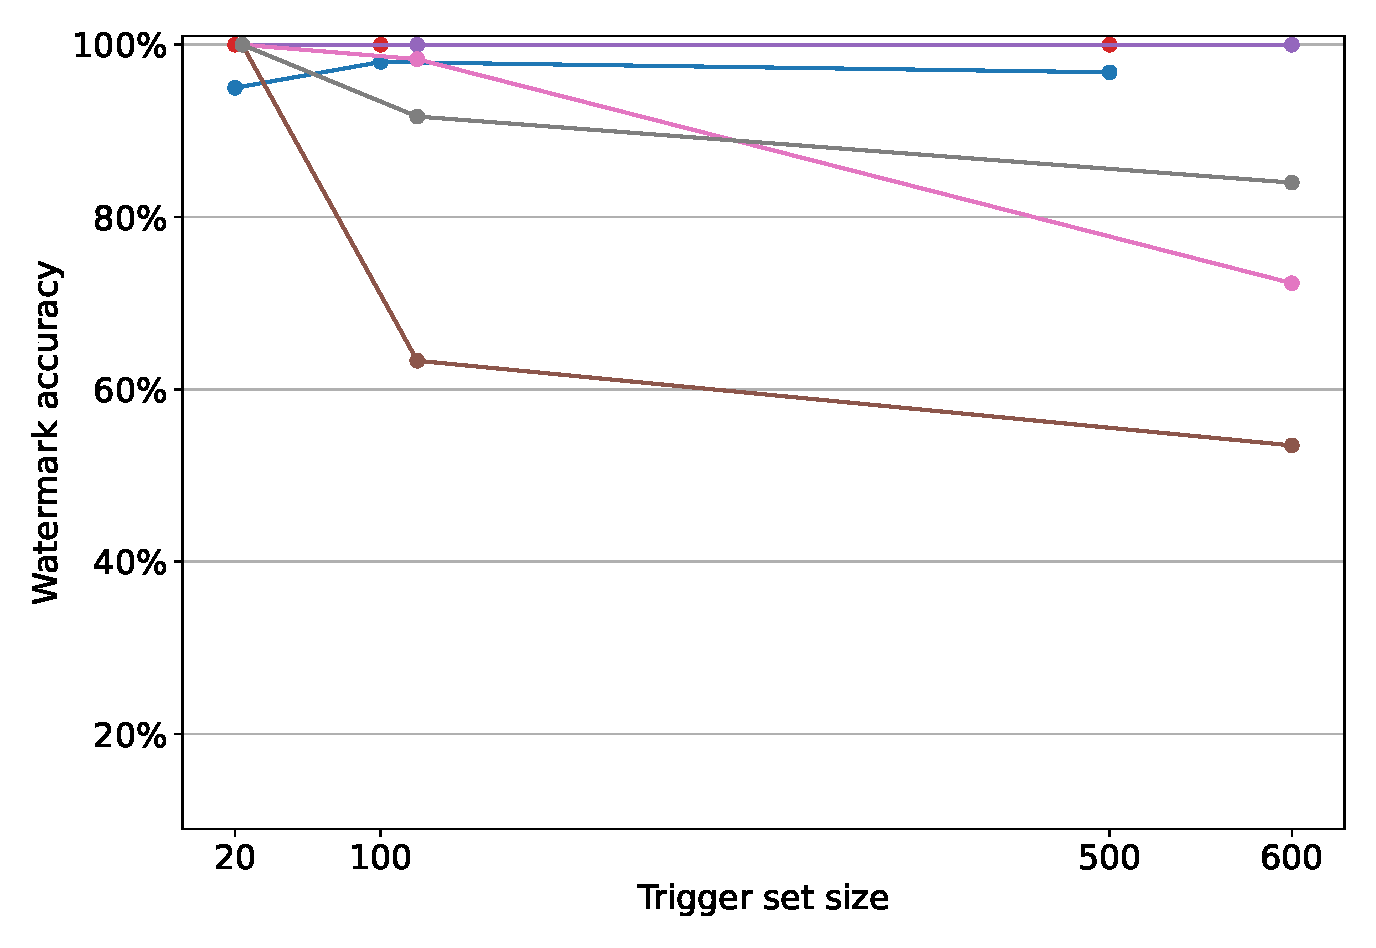
\includegraphics[width=\linewidth]{images/pruning/per_method/ProtectingIP-noise_pruning_per_method_maximal_pr_rate.eps}
        \caption{ProtectingIP-noies}
        \label{fig:pruning-max-pr-rate-noise}
    \end{subfigure}
    \quad
    \begin{subfigure}{0.4\linewidth}
        
\includegraphics[width=\linewidth]{images/pruning/per_method/PiracyResistant_pruning_per_method_maximal_pr_rate.eps}
        \caption{PiracyResistant}
        \label{fig:pruning-max-pr-rate-piracy}
    \end{subfigure}
    \quad
    \begin{subfigure}{0.4\linewidth}
        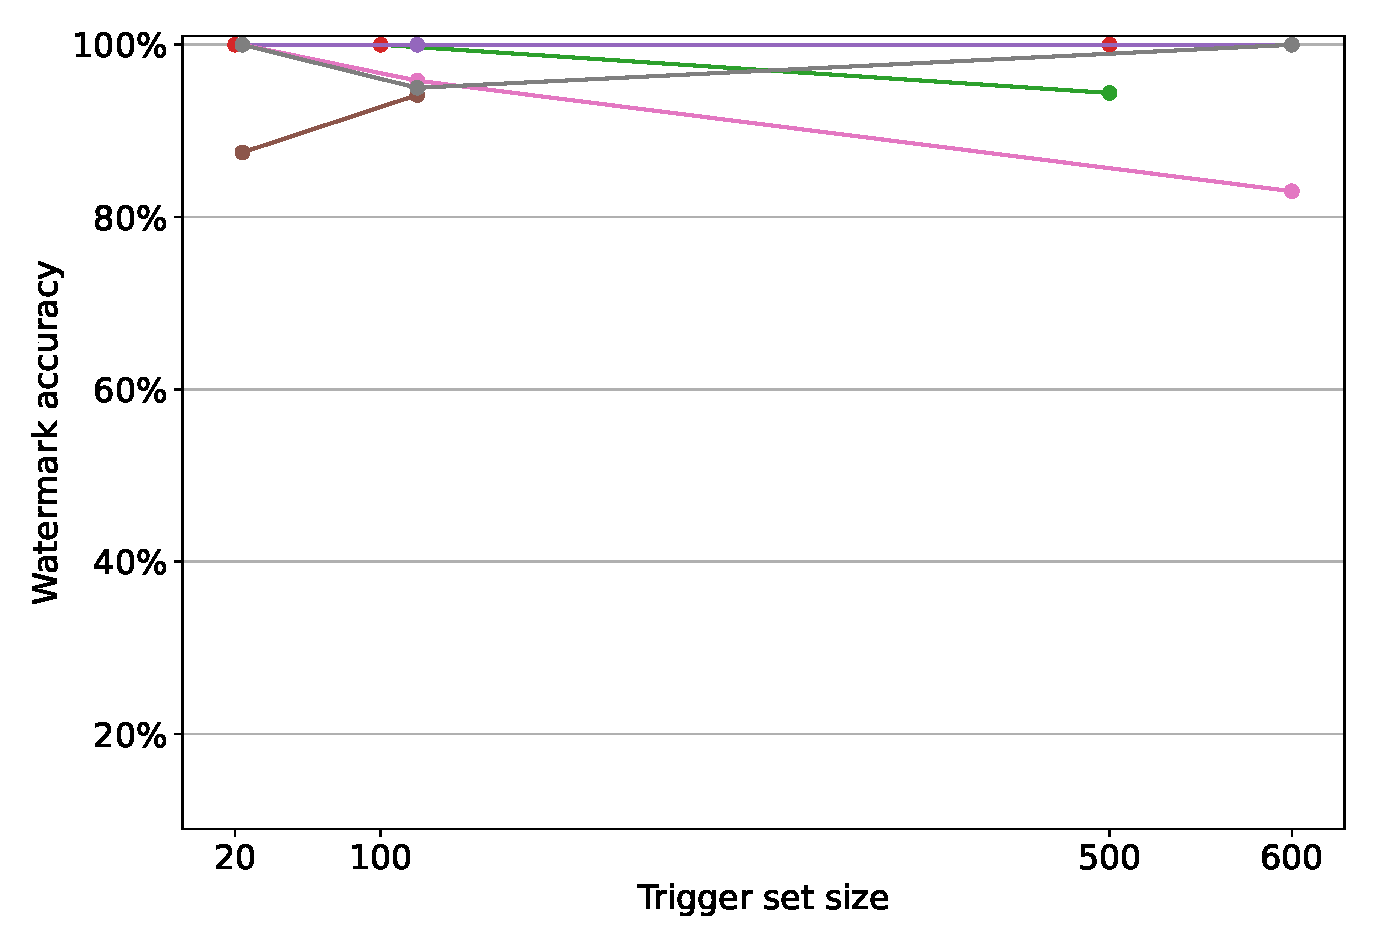
\includegraphics[width=\linewidth]{images/pruning/per_method/ExponentialWeighting_pruning_per_method_maximal_pr_rate.eps}
        \caption{ExponentialWeighting}
        \label{fig:pruning-max-pr-rate-exponential}
    \end{subfigure}
    \quad
    \begin{subfigure}{0.4\linewidth}
        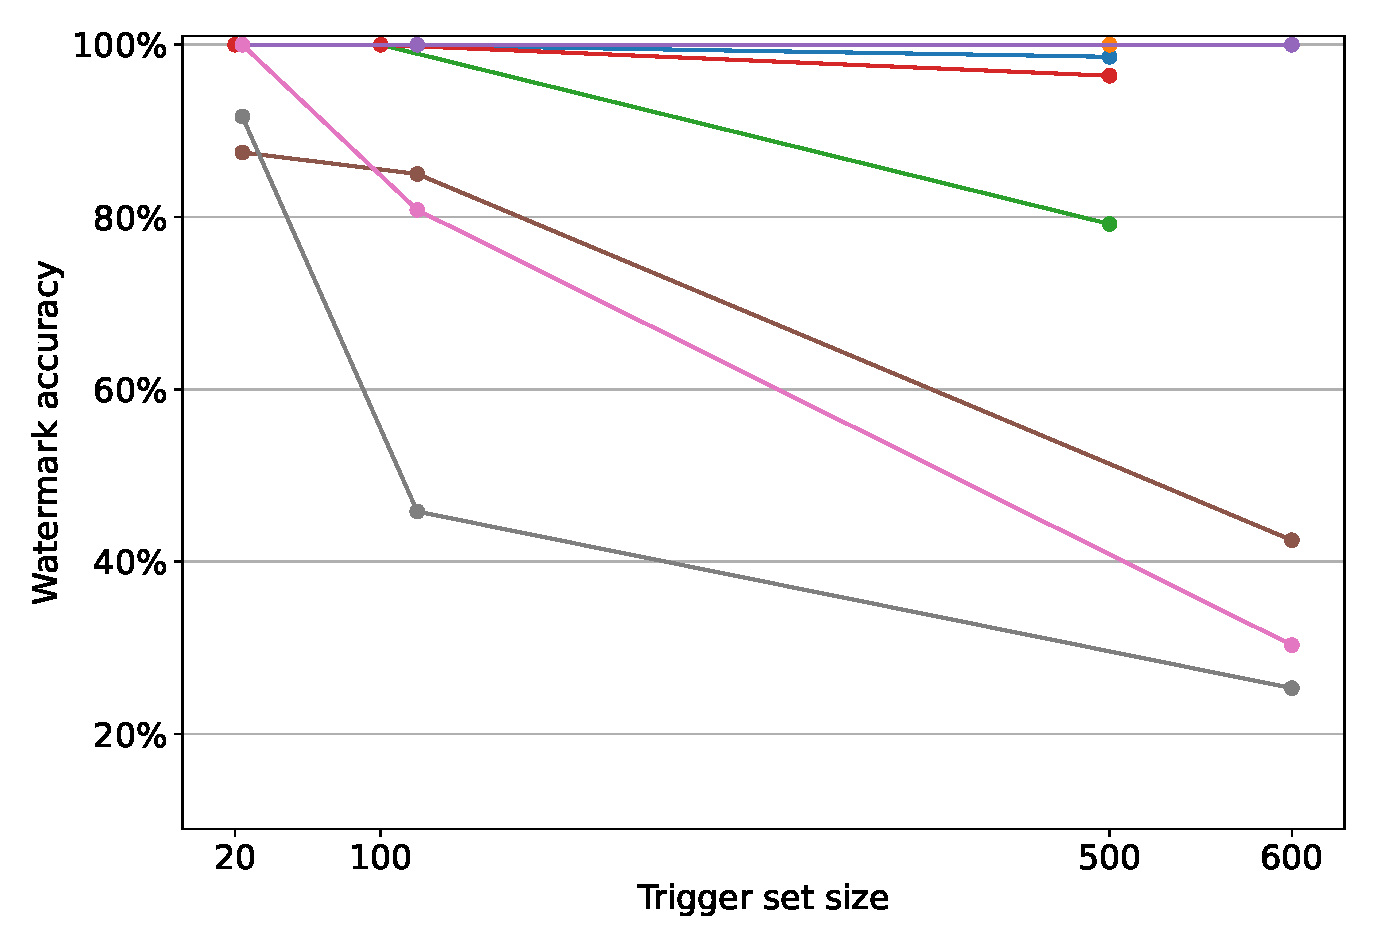
\includegraphics[width=\linewidth]{images/pruning/per_method/FrontierStitching_pruning_per_method_maximal_pr_rate.eps}
        \caption{FrontierStitching}
        \label{fig:pruning-max-pr-rate-frontier}
    \end{subfigure}
    \quad
    \begin{subfigure}{0.4\linewidth}
        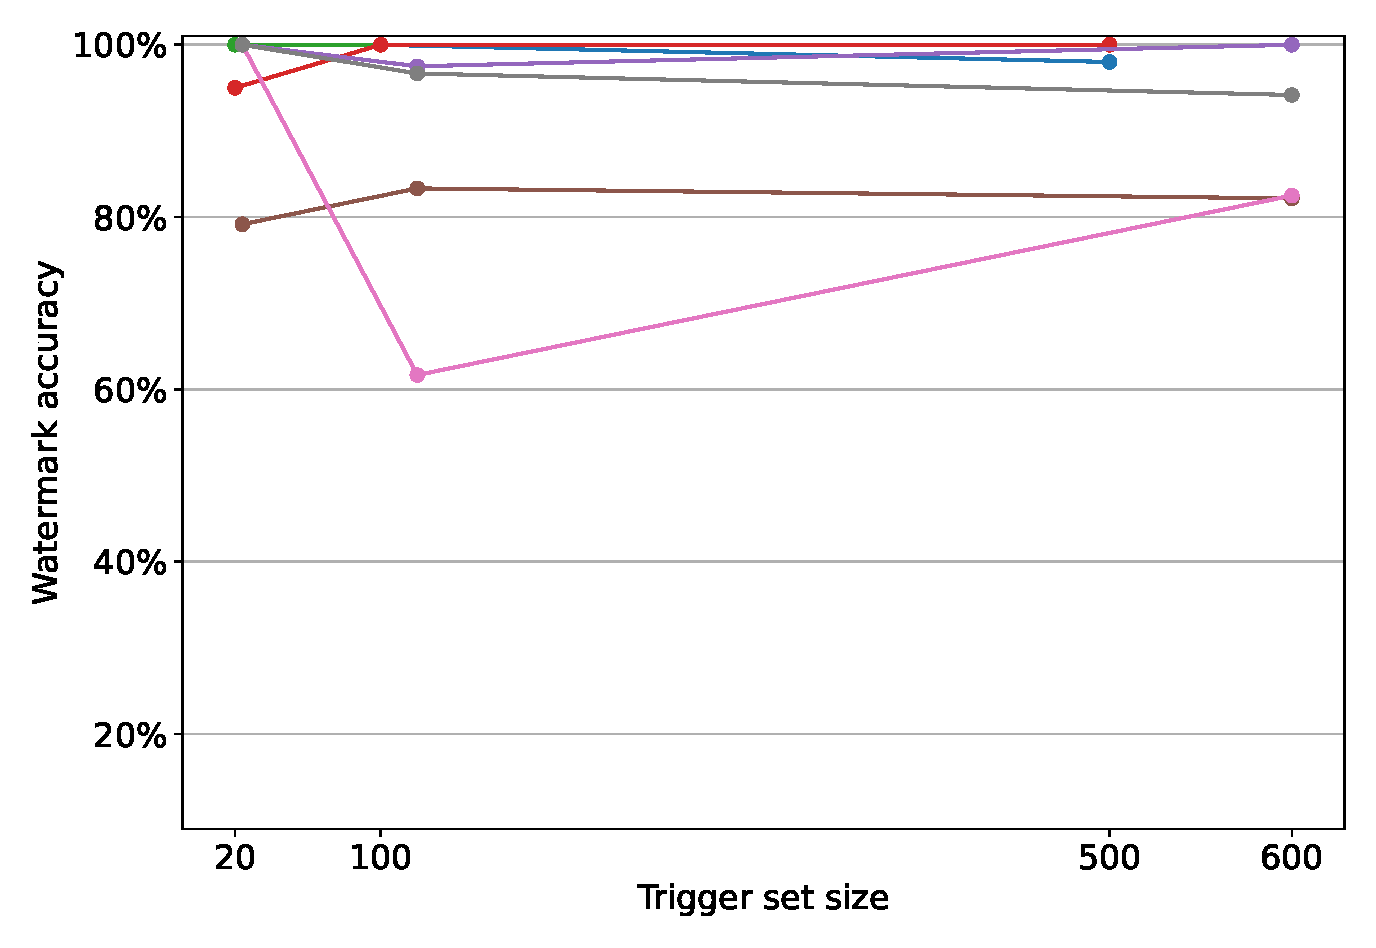
\includegraphics[width=\linewidth]{images/pruning/per_method/WMEmbeddedSystems_pruning_per_method_maximal_pr_rate.eps}
        \caption{WMEmbeddedSystems}
        \label{fig:pruning-max-pr-rate-embedded}
    \end{subfigure}
    \quad
    %\begin{subfigure}{0.4\linewidth}
    %    \includegraphics[width=\linewidth]{images/pruning/per_method/Blackmarks_pruning_per_method_maximal_pr_rate.eps}
    %    \caption{Blackmarks}
    %    \label{fig:pruning-max-pr-rate-blackmarks}
    %\end{subfigure}

    
    \begin{subfigure}{\linewidth}
    \centering
    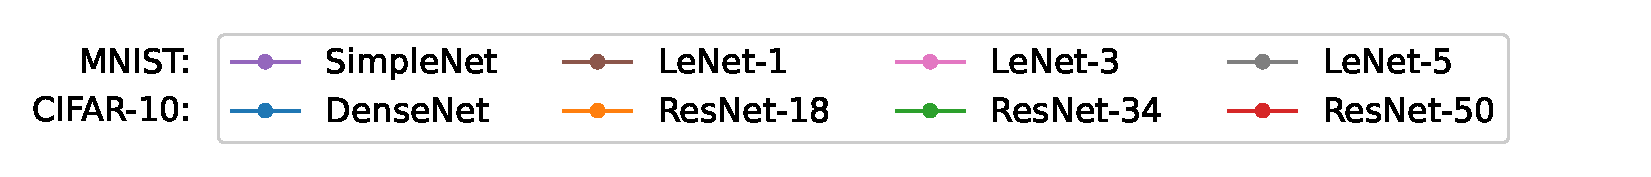
\includegraphics[width=0.7\linewidth]{images/pruning/per_method/legend_pruning_per_method_maximal_pr_rate.eps}
    \end{subfigure}
    
    \caption{Influence of the trigger set size on robustness against pruning with the maximal plausible pruning rate. Each plot corresponds to one watermarking method and shows the results for all architectures.}
    \label{fig:pruning-max-pr-rate-permethod}
\end{figure}
